%% =====================================================================
%%  Where to Go Next: Site Selection for External Validity
%%
%%  Main file.  Body sections live in sections/, proofs in appendix/.
%%  Notation and style follow the companion paper "A Sensitivity
%%  Framework for Assessing External Validity" (Boyarsky, Egami, and
%%  Namkoong 2026); shared helper packages are statistics-macros.sty,
%%  formatting.sty, editing-macros.sty.
%% =====================================================================
\documentclass[11pt]{article}

%% ---- Core typesetting ------------------------------------------------
\usepackage[margin=1in]{geometry}
\usepackage{amsmath,amssymb,amsthm,mathtools}
\usepackage{graphicx}
\usepackage[dvipsnames]{xcolor}
\usepackage{etoolbox}
\usepackage{ifthen}
\usepackage{xifthen}
\usepackage{array}
\usepackage{booktabs}
\usepackage{enumitem}
\usepackage{placeins}

%% ---- Citations (loaded before formatting.sty, which patches natbib) --
\usepackage{natbib}

%% ---- Project style helpers (order matters) --------------------------
\usepackage{statistics-macros}
\usepackage{formatting}
\usepackage{editing-macros}

%% ---- Cross-references (last) ----------------------------------------
\usepackage[colorlinks=true,allcolors=NavyBlue]{hyperref}
\usepackage[capitalize,noabbrev]{cleveref}

\crefname{assumption}{Assumption}{Assumptions}
\Crefname{assumption}{Assumption}{Assumptions}

% !TEX root = main.tex
%% ---------------------------------------------------------------------------
%% Notation shared with the companion paper "A Sensitivity Framework for
%% Assessing External Validity" (Boyarsky, Egami, and Namkoong 2026),
%% plus the site-selection objects of this paper.
%%
%% Loaded AFTER statistics-macros.sty, which supplies \E, \var, \cov,
%% \what, \R, \norm, \cp, and the theorem environments.
%% ---------------------------------------------------------------------------

\makeatletter
\@ifundefined{remark}{\newtheorem{remark}{Remark}}{}
\makeatother

%% ---- data and design (companion-paper names) -------------------------------
\newcommand{\sP}{P}                      % source law
\newcommand{\tP}{Q_T}                    % target covariate law
\newcommand{\ct}{c_T}                    % target context profile
\newcommand{\muC}{m_C}                   % E[C | X]
\newcommand{\Ctil}{\widetilde C}         % C - m_C(X)
\newcommand{\pseudo}[1]{R_{#1}}          % IPW pseudo-outcome

%% ---- omitted-moderator sensitivity ---------------------------------------
\newcommand{\Uvar}{U}                    % omitted site-level moderator
\newcommand{\uT}{u_T}                    % target moderator profile
\newcommand{\muU}{m_U}                   % E[U | X]
\newcommand{\CUcov}{\Sigma_{CU}}        % E[cov(C,U | X)]
\newcommand{\ellU}{\ell_{U,T}}           % target loading on U
\newcommand{\udisc}[1]{d_{U,#1}}         % omitted-profile contrast
\newcommand{\ovbset}{\mathcal F_U}       % omitted-moderator feasible set
\newcommand{\ovbwidth}{W_U}              % omitted-moderator interval width

%% ---- moments ---------------------------------------------------------------
\newcommand{\CovC}{\Sigma_C}             % E_P[cov(C | X)]
\newcommand{\dmom}[1]{d_{#1}}            % E_P[cov(C, R_a | X)]
\newcommand{\bT}{b_T}                    % transported baseline (scalar)
\newcommand{\ellvec}{\ell_T}             % target loading
\newcommand{\Gam}{\Gamma}                % bound inputs (b_T, ell_T, Sigma_C, d_0, d_1)

%% ---- reduced coordinates ---------------------------------------------------
\newcommand{\Vspan}{\mathcal V_C}        % span of centered site profiles
\newcommand{\Bspan}{B_C}                 % orthonormal basis of V_C
\newcommand{\Om}{\Omega}                 % B_C^T Sigma_C B_C
\newcommand{\xired}[1]{\xi_{#1}}         % B_C^T d_a

%% ---- program objects -------------------------------------------------------
\newcommand{\restrset}{\mathcal R}
\newcommand{\feasset}{\mathcal F}
\newcommand{\vminus}{v_{-}}
\newcommand{\vplus}{v_{+}}
\newcommand{\shift}{\delta}              % treatment shift beta_1 - beta_0

%% ---- site-selection objects ------------------------------------------------
\newcommand{\pool}{\mathcal S}           % existing pool of sites
\newcommand{\candset}{\mathcal K}        % candidate pool
\newcommand{\targset}{\mathcal T}        % target region
\newcommand{\cand}[1]{c^{(#1)}}          % candidate context profile
\newcommand{\newdir}[1]{u_{#1}}          % direction a candidate adds
\newcommand{\reveal}[2]{y_{#1,#2}}       % revealed scalar y_{a,k}
\newcommand{\width}{W}                   % width of the identified set
\newcommand{\affhull}{\operatorname{aff}}
\newcommand{\convhull}{\operatorname{conv}}
\providecommand{\dist}{}\renewcommand{\dist}{\operatorname{dist}}

%% ---- operators -------------------------------------------------------------
\DeclareMathOperator{\rankop}{rank}
\DeclareMathOperator{\rangeop}{range}
\DeclareMathOperator{\kernelop}{ker}
\newcommand{\range}{\rangeop}
\newcommand{\kernel}{\kernelop}
\newcommand{\pr}{\mathbb{P}}
\providecommand{\one}{\mathbf{1}}

\providecommand{\Eqref}[1]{Equation~\eqref{#1}}


\graphicspath{{figures/}}

\title{\bf Where to Go Next: Site Selection for External Validity via Sensitivity Analysis}
\date{Draft, \today}

\begin{document}
\maketitle

\begin{abstract}
A set of randomized experiments identifies the treatment effect at a new
site only in part. \citet{boyarsky2026} develop a sensitivity framework
for this problem. Under a site-level fixed-effects response model, the
observed sites determine the fixed effects only inside the span of their
centered context profiles, and the framework reports the smallest and
largest target effects consistent with the source experiments and with
restrictions the analyst states. This paper studies the natural next question. Given several candidate sites whose contexts are known but whose
experiments have not been run, which site would most strengthen the
external validity claim of the multi-site study. We show that the benefit a new site provides depends on the affine hull
of the site profiles. The target effect is
point identified exactly when the target profile lies in the affine hull
of the observed profiles, and a candidate site tightens the identified
set only if its profile lies outside that hull. We show how we can forecast the benefit that a new site provides through the vector of site-level data. We apply the method to the multi-site credit expansion data of
\citet{meager2019understanding}.
\end{abstract}


\section{Introduction}
\label{sec:intro}

Randomized experiments are often run in sites to establish evidence of an intervention applied in another site. When site-level context changes the treatment response, a
pool of internally valid experiments identifies the effect at a new site
only in part. \citet{boyarsky2026} formalize this problem. Site context
enters each potential-outcome surface through linear fixed effects, the
observed sites determine those fixed effects only inside the span of
their centered context profiles, and the target effect is reported as an
interval: the smallest and largest values consistent with the source
experiments and with restrictions the analyst is willing to state. A wide interval means that the data and the stated restrictions do not
settle the target conclusion. An infinite interval means that some
direction of extrapolation is not controlled at all.

An analyst facing a wide interval has two options. She can impose stronger restrictions, which tightens the set at the cost
of assumptions that the data cannot check. She can also collect more
evidence by running an experiment in a new site. The companion paper studies the first option.
This paper studies the second. The question is concrete because site
context is observable before any experiment is run. A funder choosing
among candidate countries already knows each country's interest rates,
loan sizes, and program rules. What she does not know is what an
experiment there would find. We ask which candidate site, if its
experiment were run, would most strengthen the external validity of the
pooled evidence, and how much of that answer is available before the
experiment.

We use the microcredit experiments harmonized by
\citet{meager2019understanding} as a running example. Seven countries ran nominally similar
expansions of credit access under very different lending terms. The
companion paper's case study holds out one country at a time and asks
what the other six imply for it. Its leave-one-out exercise shows the reverse of our question. Dropping
any one of Bosnia's six source sites leaves Bosnia's interval unsigned.
That finding also says that the sixth experiment was worth running. We ask whether an analyst who had only five
source sites could have known this in advance, from lending terms alone, and
could have chosen the right country to add.

The paper has three main findings. Each follows from the identification
geometry of the companion paper.

First, site selection is a question about the affine hull of the site
profiles. In the companion framework the observed sites identify the
fixed effects only inside the span of their centered profiles, and we
show that the target effect is point identified exactly when the target
profile lies in the affine hull of the observed profiles
(\cref{sec:geometry}). A candidate site changes what is identified only if its profile lies
outside that hull. Whether it does is checkable at design time, before
any data are collected. How far outside it lies does not matter for
identification, because any experiment along the new direction pins down
the same coordinate of the fixed effects. Distance affects precision but
not the identified set. It also affects robustness, since a farther site
is less exposed to a site-level conflict with the model.

Second, the value of a candidate experiment is computable in advance up
to one scalar per treatment arm (\cref{sec:selection}). Under the
maintained model, adding site $k$ replaces the feasible set
$\feasset$ by $\feasset$ intersected with two equality constraints,
$\newdir{k}^\top\beta_a=\reveal{a}{k}$ for $a\in\{0,1\}$, where the
direction $\newdir{k}$ is known from the candidate's context and the
scalars $\reveal{a}{k}$ are what the experiment reveals. The whole map
from those scalars to the post-addition bounds can be solved before the
experiment. Forecasting the scalars from the existing pool gives a predicted
interval, and the dual variable of the added constraint gives the effect
of a forecast error on the bounds. This is the design rule we apply in
the simulations and the case study.

Third, under the maintained model a new site can never hurt. Every width
weakly shrinks, at every target (\cref{sec:monotonicity}). This may seem
obvious, but it fails once the model is wrong. A site whose outcomes
conflict with the shared response model moves the pooled moment
conditions to a compromise between the sites. The identified slice then
translates, and the width can grow or shrink, or the program can become
infeasible. We
give an example with two source sites where one conflicting addition
doubles the width. The effect of the conflict on correctness is more important than its
effect on the width. The translated set stops covering the true effect
exactly at the targets the pool point identifies. The screens we
propose, a rank test on profiles and a compatibility check on outcomes,
separate the interior additions that refine the set from those that
corrupt it. For a site outside the hull no such check exists. We show
that a constant conflict at such a site is exactly what a different
coefficient vector would produce under the model, so the source data
cannot reveal it.

We verify each claim with the estimator the companion paper recommends,
not only with population calculations. The simulations in
\cref{sec:simulation} generate multi-site data from the fixed-effects
model, estimate the bounds with the cross-fitted rank consistent
estimator, and show that the estimated selection recovers the
population-optimal candidate in every replicate, that the design-time
predictions match the realized widths, and that the conflict mechanism
behaves as the theory says. The case study in \cref{sec:case-study}
runs the same exercise on the microcredit data. For each five-country
source pool, the rule scores the missing country from its lending terms,
and the realized experiment confirms the prediction.

\paragraph{Related work.}
The site-selection question is the forward version of the leave-one-out
exercise in the case study of \citet{boyarsky2026}, which asks which observed
sites a reported bound depends on. We ask which unobserved site a future
bound would benefit from, and we use the same three categories of what a site can do: expand
identification, add precision, or break feasibility. The problem is also related to classical optimal experimental design \citep{atkinson2007optimum,pukelsheim2006optimal}. There the
design variable is an allocation of observations inside one population
and the loss is a variance. Here the design variable is a site-level
context profile and the loss is the width of a partial-identification
interval, which variance reduction alone cannot shrink. Submodular
coverage arguments for sensor placement and subset selection
\citep{nemhauser1978analysis} appear when several sites are added at
once (\cref{sec:discussion}). Distributionally robust formulations of
worst-case effects \citep{jeong2020assessing} and structural
transportability conditions \citep{bareinboim2016causal} address what
can be learned from fixed data. Our contribution is to treat the data
that do not yet exist as the design object.

\section{Setting}
\label{sec:setting}

Throughout this paper we use the setting and sensitivity framework of \citet{boyarsky2026}. This section restates this setting.

The source sample pools $S$ sites. An observation is $O=(Y,A,X,C)$, where
$A\in\{0,1\}$ is treatment, $X$ contains unit-level covariates, and
$C\in\R^p$ is the site-level context vector, constant within a site. The
basis of $C$ is fixed before the analysis and may contain raw site
characteristics and their transformations. Site $s$ carries the profile
$c_s\in\R^p$. The source law $\sP$ mixes the sites, and treatment is
randomized within each site with known probability
$e_a(x,c)=\pr_\sP(A=a\mid X=x,C=c)$ bounded away from zero. A target site is defined by a
pair $(\tP,\ct)$: a covariate law we can sample and a context profile
$\ct\in\R^p$. Treatment and outcome data exist only for the source sites.

The framework rests on a site-level fixed-effects response model.

\begin{assumption}[Site-level fixed effects, \citealp{boyarsky2026}]
\label{ass:model}
For $a\in\{0,1\}$,
\begin{equation}
  \E_\sP[Y(a)\mid X,C]=g_a(X)+C^\top\beta_a,
  \label{eq:response-model}
\end{equation}
where $g_a$ is unrestricted and $\beta_a\in\R^p$ is fixed. Treatment is
randomized within each source site, consistency holds, the same
functions and coefficients govern the target site, and all second
moments used below are finite.
\end{assumption}

Write $\pseudo{a}=\one\{A=a\}Y/e_a(X,C)$ for the inverse-probability
pseudo-outcome, $\muC(x)=\E_\sP[C\mid X=x]$, and
$\Ctil=C-\muC(X)$. Averaging \eqref{eq:response-model} over the target
population expresses the target average treatment effect as
\begin{equation}
  \psi_T=\bT+\ellvec^\top(\beta_1-\beta_0),
  \qquad
  \begin{aligned}
    \bT&=\E_{X\sim \tP}\bigl[\E_\sP[\pseudo{1}-\pseudo{0}\mid X]\bigr],\\
    \ellvec&=\ct-\E_{X\sim \tP}\bigl[\muC(X)\bigr].
  \end{aligned}
  \label{eq:target-coefficients}
\end{equation}
The scalar $\bT$ is the covariate-transported part and is identified
under overlap in $X$. The loading $\ellvec$ multiplies the fixed-effect
contrast, which is the only unknown. Each $\beta_a$ satisfies the normal
equations of a partially linear regression \citep{robinson1988root},
\begin{equation}
  \CovC\,\beta_a=\dmom{a},
  \qquad
  \CovC=\E_\sP\bigl[\cov(C\mid X)\bigr],
  \quad
  \dmom{a}=\E_\sP\bigl[\cov(C,\pseudo{a}\mid X)\bigr].
  \label{eq:normal-equations}
\end{equation}
Because $C$ takes only $S$ values, every residual $\Ctil$ lies in the
span of the centered site profiles,
\begin{equation}
  \Vspan=\operatorname{span}\{c_s-c_1:\ s=2,\ldots,S\},
  \qquad r=\dim\Vspan\leq S-1,
  \label{eq:span}
\end{equation}
so $\range(\CovC)\subseteq\Vspan$ and $\rankop(\CovC)\leq S-1$. When
$p>S-1$ the normal equations leave fixed-effect directions undetermined,
and $\psi_T$ is point identified if and only if
$\ellvec\in\range(\CovC)$.

The key innovation of this method is that the analyst is able to encode substantive knowledge in a restriction set
$\restrset$ for the stacked vector
$\beta=(\beta_0^\top,\beta_1^\top)^\top$ as a polyhedron or a finite union
of polyhedra. \citet{boyarsky2026} provide several such candidate restrictions: magnitude caps, effect ordering, sign restrictions, and
budgets. The moments and the restriction define
\begin{equation}
  \feasset
  =\bigl\{\beta:\ \CovC\beta_a=\dmom{a},\ a\in\{0,1\},
  \ \beta\in\restrset\bigr\},
  \label{eq:feasible-set}
\end{equation}
and the sensitivity interval is $[\vminus,\vplus]$ with
\begin{equation}
  \vminus=\bT+\inf_{\beta\in\feasset}\ellvec^\top(\beta_1-\beta_0),
  \qquad
  \vplus=\bT+\sup_{\beta\in\feasset}\ellvec^\top(\beta_1-\beta_0).
  \label{eq:endpoint-programs}
\end{equation}

In this paper, we additionally define $\width=\vplus-\vminus$ as the width of the identified set at the
target. An infeasible program means the restriction contradicts the
source moments. An unbounded program means the restriction leaves a
direction that matters for the target uncontrolled. When $\width$ is a finite value it gives us a natural tool to characterize the generalizability of a particular set of experiments to a new target site.

Two more objects from \citet{boyarsky2026} are used in this paper. The
first is the reduced coordinates. Given a fixed orthonormal basis $\Bspan\in\R^{p\times
r}$ of $\Vspan$, write $\Om=\Bspan^\top\CovC\Bspan$ and
$\xired{a}=\Bspan^\top\dmom{a}$. The equality system in
\eqref{eq:feasible-set} is equivalent to
$\Om\Bspan^\top\beta_a=\xired{a}$, which has full row rank when the
smallest eigenvalue of $\Om$ is positive. We assume this eigenvalue
condition throughout, so that
$\range(\CovC)=\Vspan$ and $\kernel(\CovC)=\Vspan^\perp$. The second component is the estimator as defined by Algorithm 1. This algorithm first estimates the five inputs
$\Gam=(\bT,\ellvec,\CovC,\dmom{0},\dmom{1})$ with cross-fitted
orthogonal scores, fits $\muC$ through a joint site-probability
classifier so that every fitted residual lies in $\Vspan$ exactly, pools
the scores, and solves each bound program once in the reduced
coordinates. We call it the input-debiased estimator, in contrast to the one-step
estimator also studied in \citet{boyarsky2026}. Every estimate reported in this paper uses it.

\section{The site-selection problem}
\label{sec:problem}

\subsection{Data requirements for site-selection}
\label{subsec:problem-setup}

We assume the analyst holds data from the $S$ existing sites, which we call
the source $\pool$, and faces a candidate set $\candset=\{1,\ldots,K\}$ of
prospective sites. For each candidate $k$ we know the context profile
$\cand{k}\in\R^p$, which has same basis as the source profiles. This context is
site-level information. For example, in the \citet{meager2019understanding} dataset we use interest rates, program rules, administrative
statistics. Often these data are available from public sources before any experiment is conducted.
We also need some information about the candidate's unit-level covariate
distribution. This can often come from a census, a survey, a prior, or the assumption that units
there resemble units at a reference site. We do not have experimental results from the candidate sites, such as
treatment assignments or outcome data, because no experiment has been
conducted there.

We also state the target we care about as a set $\targset$ of context
profiles. This can be a single profile, a list of benchmark profiles,
or a box around a forecast of the target environment. A set of profiles
is enough, because the width at a target does not depend on its
covariate law (\cref{cor:width-offset}). The design
problem is
\begin{equation}
  k^\star \in \arg\min_{k\in\candset}\;
  \sup_{\ct\in\targset}\;
  \width\bigl(\ct;\ \pool\cup\{k\}\bigr),
  \label{eq:minimax}
\end{equation}
the minimax width of the identified set over the targets, evaluated as
if candidate $k$'s experiment had been run. When candidates carry
costs, as is often the case in practice, the investigator can add a cost term to the objective or screen
the pool by budget first. Everything below goes through in either case because a cost
enters separably in $k$. Choosing a
site is a discrete choice that is only made once, and it should not depend on which single target profile turns out to be the relevant one. Hence, the minimax design is a natural encoding of this problem.

The main obstacle is that $\width(\ct;\pool\cup\{k\})$ depends on data that
we do not have. The following two sections show how much we can determine via the candidate's context alone.

\subsection{What adding a site changes}
\label{subsec:augmentation}

Suppose the candidate experiment is run, with $n_k$ observations and a
randomized treatment within the site, and its data are pooled with the
existing sites. Three inputs of the bound programs change.

First, the span. The centered profile span grows from $\Vspan$ to
\begin{equation}
  \Vspan'=\Vspan+\operatorname{span}\{\cand{k}-c_1\},
  \label{eq:span-update}
\end{equation}
so its dimension rises by one when $\cand{k}-c_1\notin\Vspan$ and is
unchanged otherwise. Notice that the span update is a function of the profiles
alone. That is, we know it at ``site choice'' time.

Second, the moments. The pooled law now mixes in the candidate site, so
$\CovC$, $\dmom{a}$, $\muC$, and hence $\bT$ and $\ellvec$ all move.
Under \cref{ass:model} the new normal equations remain consistent with
the same $\beta_a$. In \cref{sec:selection} we show that their entire
effect on the feasible set is captured by one scalar per arm.

Third, the equality constraint rank. Whether the extra span direction becomes an extra rank
of $\CovC$ depends on covariate overlap. The matrix $\CovC$ averages the
conditional covariance of $C$ given $X$, and a site contributes context
variation only at covariate values where units could have come from more
than one site. A candidate whose covariate support is disjoint from the pool can
contribute profile diversity but no conditional variation. In that case
site membership is a deterministic function of $X$ on the candidate's
support, the residual $\Ctil$ vanishes there, and the added direction is
not identified. We therefore maintain the eigenvalue condition of
\cref{sec:setting} for the augmented pool: the covariance of
$\Bspan'^\top\Ctil$ has a positive smallest eigenvalue, where $\Bspan'$
is a basis of $\Vspan'$. In words, the candidate must overlap the pool
in unit-level covariates, in the same way the target must.

Throughout, the target objects $(\tP,\ct)$ are unchanged by the addition. Only the source pool grows.

\section{The geometry of adding a site}
\label{sec:geometry}

This section describes what identification looks like in the space of
site profiles. Every identification statement in the
selection problem reduces to a statement about the affine hull
\begin{equation}
  \affhull(\pool)
  =\Bigl\{\textstyle\sum_{s=1}^S w_s c_s:\ \sum_{s=1}^S w_s=1\Bigr\},
  \label{eq:affine-hull}
\end{equation}
the set of affine combinations of the observed profiles. Its direction
space is exactly $\Vspan$, the span of the centered profiles from
\eqref{eq:span}.

The first step relates the target loading to the hull. The loading
$\ellvec=\ct-\E_{\tP}[\muC(X)]$ subtracts from the target profile a
point that is always a mixture of observed profiles, because
$\muC(x)=\sum_s \pr(C=c_s\mid X=x)\,c_s$ is a convex combination of them
at every $x$. The unidentified part of the loading is therefore the part of the target
profile itself that lies outside the hull.

\begin{lemma}[The loading and the affine hull]
\label{lem:loading}
Under \cref{ass:model} and the eigenvalue condition of
\cref{sec:setting}, $\ellvec\in\range(\CovC)$ if and only if
$\ct\in\affhull(\pool)$. Moreover, for the orthogonal projection
$\Pi^\perp$ onto $\Vspan^\perp$,
\begin{equation}
  \Pi^\perp\ellvec=\Pi^\perp(\ct-c_1),
  \qquad
  \norm{\Pi^\perp\ellvec}_2=\dist\bigl(\ct,\affhull(\pool)\bigr).
  \label{eq:loading-distance}
\end{equation}
\end{lemma}

\noindent
See \cref{app:proofs} for all proofs. \cref{lem:loading} turns the point-identification condition of the
companion paper into a statement an investigator can check from the
profiles alone. The pooled experiments determine the target effect
exactly when the target's context is an affine combination of the
observed contexts. The relevant set is the affine hull, not the convex
hull. A target outside the convex hull but inside the affine hull is
still point identified, because the fixed effects are linear in context,
so the model allows linear extrapolation along observed directions.
Identification fails only in a direction that no combination of observed
sites reaches.

The same projection governs the width under any restriction. On the
feasible set the projection of the treatment shift onto $\Vspan$ is
fixed, so only the part of the loading outside $\Vspan$ can move the
objective.

\begin{corollary}[The width depends on the target only through its offset]
\label{cor:width-offset}
Under the conditions of \cref{lem:loading} and for any restriction set
$\restrset$, the width $\width$ of \eqref{eq:endpoint-programs} depends
on the target $(\tP,\ct)$ only through $\Pi^\perp(\ct-c_1)$. In
particular it does not depend on the target covariate law $\tP$.
\end{corollary}

\noindent
The endpoints themselves do depend on $\tP$ through $\bT$ and the
in-span part of $\ellvec$, but both endpoints move by the same amount.
\cref{cor:width-offset} is what justifies writing the width as
$\width(\ct;\pool)$ and stating the target region below as a set of
profiles.

Without restrictions, partial identification in the response model
reduces to a dichotomy. \citet{boyarsky2026} formalize this.

\begin{proposition}[Unrestricted dichotomy]
\label{prop:dichotomy}
Let $\restrset=\R^{2p}$. Under the conditions of \cref{lem:loading},
\begin{equation}
  \width(\ct;\pool)=
  \begin{cases}
    0 & \text{if } \ct\in\affhull(\pool),\\
    +\infty & \text{otherwise.}
  \end{cases}
  \label{eq:dichotomy}
\end{equation}
\end{proposition}

\noindent
With $\restrset=\R^{2p}$ the program is always feasible under the model,
since $\beta^\circ$ satisfies the moment equations, so the width is never
undefined.

A candidate site enters this geometry through one object only, the
direction its profile adds to the span.

\begin{proposition}[Span expansion is affine-hull expansion]
\label{prop:hull}
Let $\newdir{k}$ be the component of $\cand{k}-c_1$ orthogonal to
$\Vspan$. Then $\Vspan'$ of \eqref{eq:span-update} satisfies
$\dim\Vspan'=r+1$ if and only if $\newdir{k}\neq0$, which holds if and
only if $\cand{k}\notin\affhull(\pool)$. In that case
$\Vspan'^{\perp}=\Vspan^\perp\cap\{\newdir{k}\}^\perp$, and under the
augmented eigenvalue condition of \cref{subsec:augmentation} the
augmented covariance satisfies $\range(\CovC')=\Vspan'$ and
$\kernel(\CovC')=\Vspan'^\perp$. If instead
$\cand{k}\in\affhull(\pool)$, the span, the range, and the kernel are
unchanged.
\end{proposition}

Together with \cref{prop:dichotomy}, this gives the unrestricted
selection rule. A candidate collapses an infinite width at target $\ct$
to zero exactly when the target's offset from the hull,
$\Pi^\perp(\ct-c_1)$, is a nonzero multiple of $\newdir{k}$. When the
offsets of the targets span two or more directions outside $\Vspan$, no
single candidate gives point identification, and every candidate leaves
the unrestricted minimax width at $+\infty$. The unrestricted rule then
cannot rank candidates, which is one reason the selection problem needs
restrictions. Only the direction of $\newdir{k}$ enters. How far outside the hull the candidate sits does
not change what becomes identified, because a fixed-effects model pins
the same coefficient combination from a small step along a direction as
from a large one. Distance along the new direction affects the precision of the added
constraint, through the context variance the new site contributes. A
farther site therefore improves precision but not identification.

Restrictions replace the dichotomy with finite widths. In that case the
distance from the target to the hull is the right continuous measure of
what remains unidentified. The simplest statement uses a cap on the size
of the treatment shift $\shift=\beta_1-\beta_0$.

\begin{proposition}[Width equals distance under a norm cap]
\label{prop:distance}
Let the restriction be $\norm{\shift}_2\leq\tau$ with no restriction on
$\beta_0$, let $\bar\shift$ be the minimum-norm solution of
$\CovC\shift=\dmom{1}-\dmom{0}$, and assume
$\tau\geq\norm{\bar\shift}_2$. Under the conditions of
\cref{lem:loading},
\begin{equation}
  \width(\ct;\pool)
  =2\sqrt{\tau^2-\norm{\bar\shift}_2^2}\;
  \dist\bigl(\ct,\affhull(\pool)\bigr).
  \label{eq:width-distance}
\end{equation}
\end{proposition}

\noindent
The same formula holds for the augmented pool, with two changes. The
distance is to $\affhull(\pool\cup\{k\})$, and the minimum-norm shift
becomes $\Pi_{\Vspan'}\shift^\circ$, where $\shift^\circ$ is the true
shift. Writing $\newdir{k}$ with unit length,
\begin{equation}
  \width(\ct;\pool\cup\{k\})
  =2\sqrt{\tau^2-\norm{\bar\shift}_2^2-(\newdir{k}^\top\shift^\circ)^2}\;
  \dist\bigl(\ct,\affhull(\pool\cup\{k\})\bigr),
  \label{eq:width-distance-aug}
\end{equation}
provided the true shift satisfies the cap (\cref{app:proof-distance}).
The first factor depends on the candidate through the unknown scalar
$\newdir{k}^\top\shift^\circ=\reveal{1}{k}-\reveal{0}{k}$ that its
experiment reveals. So under this restriction the ranking of candidates
by \eqref{eq:minimax} is not a ranking by distance alone. Two statements
do hold before the experiment. First, at the neutral forecast of
\cref{sec:selection}, which sets this scalar to zero, the first factor is
the same for every candidate, and the minimax rule chooses the candidate
whose profile, added to the hull, leaves no target in $\targset$ far
from it. Second, because the first factor is largest at zero, the
width at the neutral forecast is an upper bound on each candidate's
realized width under this restriction.

\section{Scoring candidates under restrictions}
\label{sec:selection}

Applied bounds are computed under substantive restrictions, so the selection rule must handle a polyhedral $\restrset$, where widths
are finite and the dichotomy of \cref{prop:dichotomy} no longer holds. The
key structural fact is that the candidate's entire effect on the
feasible set passes through two scalars.

\begin{proposition}[Adding a site adds two equality constraints]
\label{prop:refinement}
Suppose \cref{ass:model} holds for the pool and for candidate $k$, and
the eigenvalue condition holds for the augmented pool. Let
$\feasset'$ denote the feasible set \eqref{eq:feasible-set} built from
the augmented moments. If $\cand{k}\notin\affhull(\pool)$, then, with
$\newdir{k}$ normalized to unit length,
\begin{equation}
  \feasset'
  =\feasset\cap
  \bigl\{\beta:\ \newdir{k}^\top\beta_a=\reveal{a}{k},\ a\in\{0,1\}\bigr\},
  \qquad
  \reveal{a}{k}=\newdir{k}^\top\beta_a,
  \label{eq:refinement}
\end{equation}
where $\reveal{a}{k}$ is identified by the augmented pool but not by
$\pool$. If $\cand{k}\in\affhull(\pool)$, then $\feasset'=\feasset$.
The bounds \eqref{eq:endpoint-programs} built from the augmented moments
equal the bounds built from the base objective $(\bT,\ellvec)$ over
$\feasset'$: the changes in $\bT$ and $\ellvec$ induced by re-pooling
shift both endpoints by the same amount tied to the re-decomposition of
$\psi_T$, and the target effect interval is unchanged by them.
\end{proposition}

\cref{prop:refinement} is the basis of the design rule. The direction
$\newdir{k}$ is computable from the profiles before the experiment. The scalars
$\reveal{0}{k}$ and $\reveal{1}{k}$ are what the candidate experiment
reveals: the projection of each arm's fixed effects on the new
direction. Everything else about the candidate's data (its sample size, its noise
level, and its covariate mix) affects only how precisely those two
scalars are estimated. It does not affect the identified set.

\paragraph{The predicted interval.}
Define the design-time width map
\begin{equation}
  \width_k(\ct;\,y_0,y_1)
  =\text{width of \eqref{eq:endpoint-programs} over }
  \feasset\cap\{\newdir{k}^\top\beta_a=y_a,\ a\in\{0,1\}\},
  \label{eq:width-map}
\end{equation}
a pair of linear programs the investigator can solve before the
experiment, for any conjectured $(y_0,y_1)$. Before the experiment we evaluate it at a
forecast. The neutral forecast extends the pool's own fit. The minimum-norm
solution $\what\beta_a$ of the estimated equality system sets the
unidentified coordinates to zero, so its forecast is
$\what y_a=\newdir{k}^\top\what\beta_a=0$. Any substantive prior that
maps the candidate's context to expected outcomes can replace it. We
call $\width_k(\ct;\what y_0,\what y_1)$ the predicted width and use it,
maximized over $\targset$, as the score in \eqref{eq:minimax}.

\paragraph{Pricing the forecast error.}
The prediction is wrong only to the extent that the forecast is wrong.
The sensitivity follows from a standard envelope argument. At a bound
with a unique optimizer and dual, the derivative of the bound in $y_a$
is the multiplier on the added row, so for small errors
\begin{equation}
  v_j(y)\approx v_j(\what y)
  +\sum_{a\in\{0,1\}}\lambda^{u}_{j,a}\,(y_a-\what y_a),
  \qquad j\in\{-,+\},
  \label{eq:dual-pricing}
\end{equation}
where $\lambda^{u}_{j,a}$ is bound $j$'s dual variable on the constraint
$\newdir{k}^\top\beta_a=y_a$. This is the same envelope argument that the inference theory of the
companion paper uses, applied to the added rows. An investigator who can bound the forecast error, say
$|y_a-\what y_a|\leq B$, obtains a range of predicted intervals by
adding $\sum_a(|\lambda^{u}_{-,a}|+|\lambda^{u}_{+,a}|)\,B$ to the
predicted width, or exactly by re-solving \eqref{eq:width-map} on a grid
of $y$ values, since the map is piecewise linear in $y$. In our
simulations and in the case study the ranking of candidates is stable
across these variants, because the ranking depends on which direction is resolved and not on
the forecast level.

\paragraph{Three kinds of candidate.}
The three categories from the companion paper's leave-one-out exercise
also describe what a candidate can do.
\begin{itemize}
\item \emph{Identification.} If $\cand{k}\notin\affhull(\pool)$, the
  candidate adds the equality constraints \eqref{eq:refinement}. This is
  the only way a candidate changes the identified set, and it is
  checkable from profiles alone.
\item \emph{Precision.} If $\cand{k}\in\affhull(\pool)$, the identified
  set is unchanged, and the candidate's value is statistical. More context
variation inside $\Vspan$ tightens the estimates and the standard errors
of the same bounds. Interior sites add precision but not identification.
\item \emph{Feasibility.} A candidate can also restore or destroy
  feasibility. If the pool's program is infeasible under $\restrset$,
  no addition restores it, since $\feasset'\subseteq\feasset$ under the
  model. But an addition whose data conflict with the model can make a feasible
program infeasible. An infeasible augmented program then signals that
conflict, not a property of the candidate.
  \cref{sec:monotonicity} takes this up.
\end{itemize}

\paragraph{Scoring procedure.}
The rule we use in \cref{sec:simulation,sec:case-study} has four steps.
\begin{enumerate}
\item For each candidate, test $\cand{k}$ against $\affhull(\pool)$.
\item For each candidate that expands the hull, solve \eqref{eq:width-map}
  at the forecast over $\targset$.
\item Report the minimax score, the resolved direction, and the dual
  prices of the forecast.
\item Break ties, and rank interior candidates, by predicted precision
  at fixed identification.
\end{enumerate}
The whole computation reuses the base-pool estimate $\what\Gam$ and adds two rows per
candidate, so scoring a pool of $K$ candidates costs $K$ pairs of linear
programs per target beyond the base fit.

\section{When adding a site can hurt}
\label{sec:monotonicity}

One might hope that new evidence can only help, so that the design
problem is only about how much a candidate helps. Under the maintained
model this is true.

\begin{theorem}[Monotone improvement under the model]
\label{thm:monotone}
Suppose \cref{ass:model} holds for the pool and for candidate $k$, the
augmented eigenvalue condition holds, and the true coefficient vector
satisfies $\beta\in\restrset$. Then $\feasset'\subseteq\feasset$, both
sets contain $\beta$, and for every target $\ct$,
\begin{equation}
  \width(\ct;\pool\cup\{k\})\;\leq\;\width(\ct;\pool),
  \label{eq:monotone}
\end{equation}
with equality for every target when $\cand{k}\in\affhull(\pool)$. In
particular the augmented program is feasible and its interval still
contains the true target effect $\psi_T$.
\end{theorem}

The assumptions of \cref{thm:monotone} show where it can fail. Every
assumption is a modeling commitment about the new site. The new site
must share the response surfaces $g_a$ and the fixed effects $\beta_a$
of \eqref{eq:response-model}. A site that does not share them, e.g.,
because its implementation or its measurement differs, moves the pooled
normal equations. The normal equations then average conflicting
site-level means, and the identified slice of coefficient space
translates to a compromise that fits no site exactly. The restriction set then cuts the
translated slice at a different cross-section, and the width can move
either way.

\paragraph{A two-site example.}
Take one context coordinate pair, $p=2$, and two source sites with
profiles $c_1=(0,0)$ and $c_2=(1,1)$, the two-site configuration
\citet{boyarsky2026} use to illustrate partial identification. The pool identifies one combination of the
treatment shift, $\delta_1+\delta_2=2$ say, and leaves the direction
$(1,-1)$ free. Impose the box $\shift\in[0,2]\times[-1,1]$ and take a
target that loads on $\delta_1$ alone. The feasible segment is
$\{(\delta_1,2-\delta_1):\delta_1\in[1,2]\}$ and the width is $1$. Now
add a third site on the same line through the profiles whose experiment
implies $\delta_1+\delta_2=0$, in conflict with the pool. Pooling the
two inconsistent moment conditions with equal weight moves the
identified value of $\delta_1+\delta_2$ to the compromise $1$. The new
feasible segment is $\{(\delta_1,1-\delta_1):\delta_1\in[0,2]\}$ and the
width is $2$. A rank-preserving addition doubled the width without changing the
restriction set. Panel (A) of \cref{fig:monotonicity}
draws this example.

\paragraph{What conflict corrupts first.}
Width is not the right measure of the damage. The translated slice can
just as easily cut a narrower cross-section of the restriction set, in
which case the conflicted pool reports a tighter interval around a wrong
location. The precise statement concerns whether the interval covers the true
effect. The translation moves the point the pool identifies, so the
targets that suffer first are the point-identified ones. Their intervals
have width zero, so any movement removes the true effect from the
interval. A wide interval can still cover the true effect after a small
conflict. A point prediction cannot. In the simulation of
\cref{sec:simulation} the conflicted addition changes the worst-case
width by only a few percent in either direction, while the population
interval stops covering the true effect at the span-identified targets
in every replicate. An analyst who sees a surprisingly tight interval after pooling a new
site should treat it as a sign of conflict rather than as an
improvement.

\paragraph{Screens.}
Two checks separate refining additions from corrupting ones.
\begin{itemize}
\item \emph{Rank screen, before the experiment.} Test
  $\cand{k}\notin\affhull(\pool)$. A candidate that passes adds the
  equality constraints \eqref{eq:refinement} and, under the model,
  cannot widen anything (\cref{thm:monotone}). A candidate that fails
  changes no identified quantity, so any movement of the estimated set
  after adding it, beyond sampling noise, is itself evidence of
  conflict.
\item \emph{Compatibility screen, after the experiment.} The candidate's
  data overidentify the in-span coordinates: the projections
  $\Bspan^\top\beta_a$ are estimated by the pool and, once the
  experiment runs, by the candidate site jointly with the pool. Compare
  the pool's minimum-norm fit with the augmented fit on the in-span
  coordinates, in units of their standard errors. A large discrepancy indicates the conflict mechanism above. The check is
an overidentification test of the kind used to detect an invalid
instrument. The forecast
  version of this screen, before the experiment, compares the
  candidate's predicted outcomes under the pool's fit with whatever
  prior information exists about outcomes there.
\end{itemize}
When a screen fails, the analyst should report both analyses, the bounds
with and without the new site, together with the discrepancy between
them. Dropping the new site assumes that the pool is right. Pooling
assumes that the model is right. The screens make the disagreement
visible so the analyst can decide which assumption to keep.

\section{Site selection for omitted moderators}
\label{sec:omitted-moderator}

The fixed-effects response model is a statement about which site-level
variables modify the response. It can fail because a relevant moderator is
omitted from $C$. Omitted-variable bias is especially useful here because it
separates two quantities that are often conflated: the strength of the omitted
moderator in the treatment effect and the extent to which the moderator is
imbalanced between the source sites and the target.

Let $U\in\R^q$ be a site-level moderator with profile $u_s$ at site $s$.
For this section, suppose the treatment-effect contrast obeys the augmented
response model
\begin{equation}
  \E_\sP[Y(1)-Y(0)\mid X,C,U]
  =g_\Delta(X)+C^\top\theta+U^\top\gamma,
  \qquad
  \theta=\beta_1-\beta_0,
  \label{eq:omitted-response-model}
\end{equation}
where $\gamma\in\R^q$ is the effect of the omitted moderator. The analysis in
the rest of the paper fits the model without $U$. Define
\begin{equation}
  \muU(x)=\E_\sP[U\mid X=x],
  \qquad
  \CUcov=\E_\sP[\cov(C,U\mid X)],
  \qquad
  \ellU=\uT-\E_{X\sim\tP}[\muU(X)].
  \label{eq:omitted-objects}
\end{equation}
The target now has an omitted-moderator profile $\uT$. These quantities need
not be observed; they index the sensitivity analysis.

\begin{proposition}[Omitted-moderator bias]
\label{prop:omitted-bias}
Let $\theta^C$ solve the normal equations from fitting the response model
without $U$, so that
\begin{equation}
  \CovC\theta^C=\dmom{1}-\dmom{0}.
  \label{eq:omitted-normal-equation}
\end{equation}
Under \eqref{eq:omitted-response-model},
\begin{equation}
  \dmom{1}-\dmom{0}=\CovC\theta+\CUcov\gamma.
  \label{eq:omitted-moment-shift}
\end{equation}
If $\ct\in\affhull(\pool)$, then the target value reported by the
misspecified model, $\psi_T^C=\bT+\ellvec^\top\theta^C$, differs from the
true target effect by
\begin{equation}
  \psi_T-\psi_T^C
  =\bigl(\ellU-\ellvec^\top\CovC^\dagger\CUcov\bigr)^\top\gamma.
  \label{eq:omitted-bias}
\end{equation}
\end{proposition}

The two terms in \eqref{eq:omitted-bias} have a direct interpretation. The
loading $\ellU$ is the source--target difference in the omitted moderator,
while $\ellvec^\top\CovC^\dagger\CUcov$ is the component that the fitted
context coefficients absorb because $U$ is associated with $C$ in the source
pool. The formula is invariant to the choice of solution $\theta^C$ because
$\ellvec\in\range(\CovC)$ when the target is in the affine hull.

The same decomposition gives a new role to sites that are interior in the
observed context geometry. Let a candidate satisfy
$\cand{k}=\sum_s w_s c_s$ with $\sum_s w_s=1$, and define its omitted-profile
contrast
\begin{equation}
  \udisc{k}=u_k-\sum_s w_su_s.
  \label{eq:omitted-direction}
\end{equation}
The weights may be negative, as they are for affine, rather than convex,
combinations. If $\udisc{k}\neq0$, the candidate is outside the affine hull
of the existing profiles in the augmented $(C,U)$ space even though it is
inside the affine hull in $C$ alone. It therefore tests a direction that the
maintained model treats as irrelevant.

\begin{theorem}[Refinement under an omitted moderator]
\label{thm:omitted-refinement}
Suppose the augmented response model \eqref{eq:omitted-response-model} holds
for the source pool and candidate $k$. Let $\rho_k$ denote the population
contrast between the candidate's conditional treatment effect and the same
affine combination of source-site conditional treatment effects. Then, for
every $x$,
\begin{equation}
\begin{split}
\rho_k
&=\E[Y(1)-Y(0)\mid X=x,C=\cand{k},U=u_k]\\
&\quad-\sum_s w_s\E[Y(1)-Y(0)\mid X=x,C=c_s,U=u_s]
=\udisc{k}^\top\gamma.
\end{split}
\label{eq:omitted-contrast}
\end{equation}
Consider an omitted-moderator sensitivity set
\begin{equation}
  \ovbset
  =\bigl\{(\theta,\gamma):\CovC\theta+\CUcov\gamma
  =\dmom{1}-\dmom{0},\ (\theta,\gamma)\in\restrset_U\bigr\},
  \label{eq:omitted-feasible-set}
\end{equation}
and the target functional
\begin{equation}
  \psi_T(\theta,\gamma)
  =\bT+\ellvec^\top\theta+\ellU^\top\gamma.
  \label{eq:omitted-target-functional}
\end{equation}
After the candidate experiment is observed, the feasible set is
\begin{equation}
  \ovbset^{(k)}
  =\ovbset\cap\bigl\{(\theta,\gamma):\udisc{k}^\top\gamma=\rho_k\bigr\}.
  \label{eq:omitted-feasible-update}
\end{equation}
If the true $(\theta,\gamma)$ belongs to $\ovbset$, then the corresponding
identified-set width satisfies, for every target,
\begin{equation}
  \ovbwidth(\ct,\uT;\pool\cup\{k\})
  \leq \ovbwidth(\ct,\uT;\pool).
  \label{eq:omitted-monotonicity}
\end{equation}
If $\udisc{k}=0$, then $\rho_k=0$ and the candidate adds no omitted-moderator
restriction, so the two widths are equal. If $\udisc{k}\neq0$, the candidate
can strictly reduce the width whenever the restriction
$\udisc{k}^\top\gamma=\rho_k$ cuts a target-relevant direction in $\ovbset$.
\end{theorem}

The theorem is the omitted-variable analogue of \cref{thm:monotone}. Under the
maintained model, a candidate outside the observed affine hull is valuable
because it identifies a new context direction. Under the augmented model, an
interior candidate is valuable when it is outside the affine hull after the
omitted moderator is included. The design criterion is therefore to seek
sites for which $\udisc{k}$ is large in directions of $\gamma$ that matter for
$\ellU$. If $U$ is not measured, this direction must be supplied by a proxy,
substantive prior, or sensitivity range. Without such information, an
unrestricted omitted moderator remains unconstrained by any site-selection
rule based on $C$ alone.

\section{Simulations}
\label{sec:simulation}

We check the theory with the estimator a user would run, not only with
population calculations. Both experiments generate multi-site data
from the fixed-effects model \eqref{eq:response-model}, estimate the
five bound inputs with the rank consistent estimator of
\citet{boyarsky2026}, and solve the estimated bound programs. The
replication code reproduces every number and figure.

\subsection{Design}
\label{subsec:sim-design}

The context space has $p=6$ coordinates. Six existing sites carry fixed
profiles whose centered span $\Vspan$ has rank three, so three
directions of the fixed effects are unidentified, the same mechanism as
in the microcredit data. Each site contributes 500 observations with
three unit-level covariates, a binary covariate, a discrete covariate
whose distribution varies by site, and a Gaussian covariate. Treatment
probabilities are known and vary by site between $0.35$ and $0.65$. An
independent target covariate sample has 1{,}500 observations. The
target region $\targset$ holds fifteen fixed profiles, five inside the
affine hull of the pool and ten with components outside it. The
restriction is the per-arm box $|\beta_{a,j}|\leq 2.5$, which keeps
every width finite and contains the truth with room to spare. Estimation
uses four folds and correctly specified linear and multinomial logistic
nuisance fits, so the experiments isolate the selection problem rather
than nuisance error. Exact population moments and widths come from
finite enumeration of the discrete covariates. Each experiment runs 40
replicates that redraw the data with the geometry fixed.

\subsection{Selecting among four candidates}
\label{subsec:sim-selection}

Four candidate sites cover the three categories of \cref{sec:selection}: $k_1$
inside the convex hull of the existing profiles, $k_2$ inside the affine
hull but outside the convex hull, and $k_3$ and $k_4$ outside the
affine hull along two different directions, $k_3$ far outside along the
first and $k_4$ a short step along the second. For each candidate we
compute the design-time prediction from the existing pool alone, then
simulate the candidate experiment from the same model, refit the
estimator on the seven-site pool, and record the realized worst-case
width over $\targset$.

\Cref{fig:selection} reports the results. The population worst-case
width is $18.31$ for the existing pool and stays exactly $18.31$ when
$k_1$ or $k_2$ is added: sites inside the affine hull change nothing
about identification, whether or not they are inside the convex hull.
The two hull-expanding candidates cut the population worst-case width to
$14.63$ ($k_3$) and $13.54$ ($k_4$), reductions of 20 and 26 percent.
The estimated widths track the population values to within sampling
noise in every cell, with mean estimates of $18.31$, $18.31$, $18.29$,
$14.63$, and $13.59$. The estimated selection picks $k_4$, the
population-optimal candidate, in all 40 replicates, and so does the
design-time selection computed before the candidate data exist. The
design-time predictions are conservative, $16.49$ against a realized
$14.63$ for $k_3$ and $14.04$ against $13.59$ for $k_4$, because the
neutral forecast slices the restriction box through its widest
cross-section, and they preserve the ranking.

The comparison between $k_3$ and $k_4$ makes the geometry of
\cref{sec:geometry} concrete. The nearby candidate beats the distant
one because the worst-case targets load more on the direction $k_4$
resolves than on the direction $k_3$ resolves. Distance to the hull does not enter the identified set. The identified
set depends on which direction a candidate resolves and how much the
target region loads on it.

\begin{figure}[t]
  \centering
  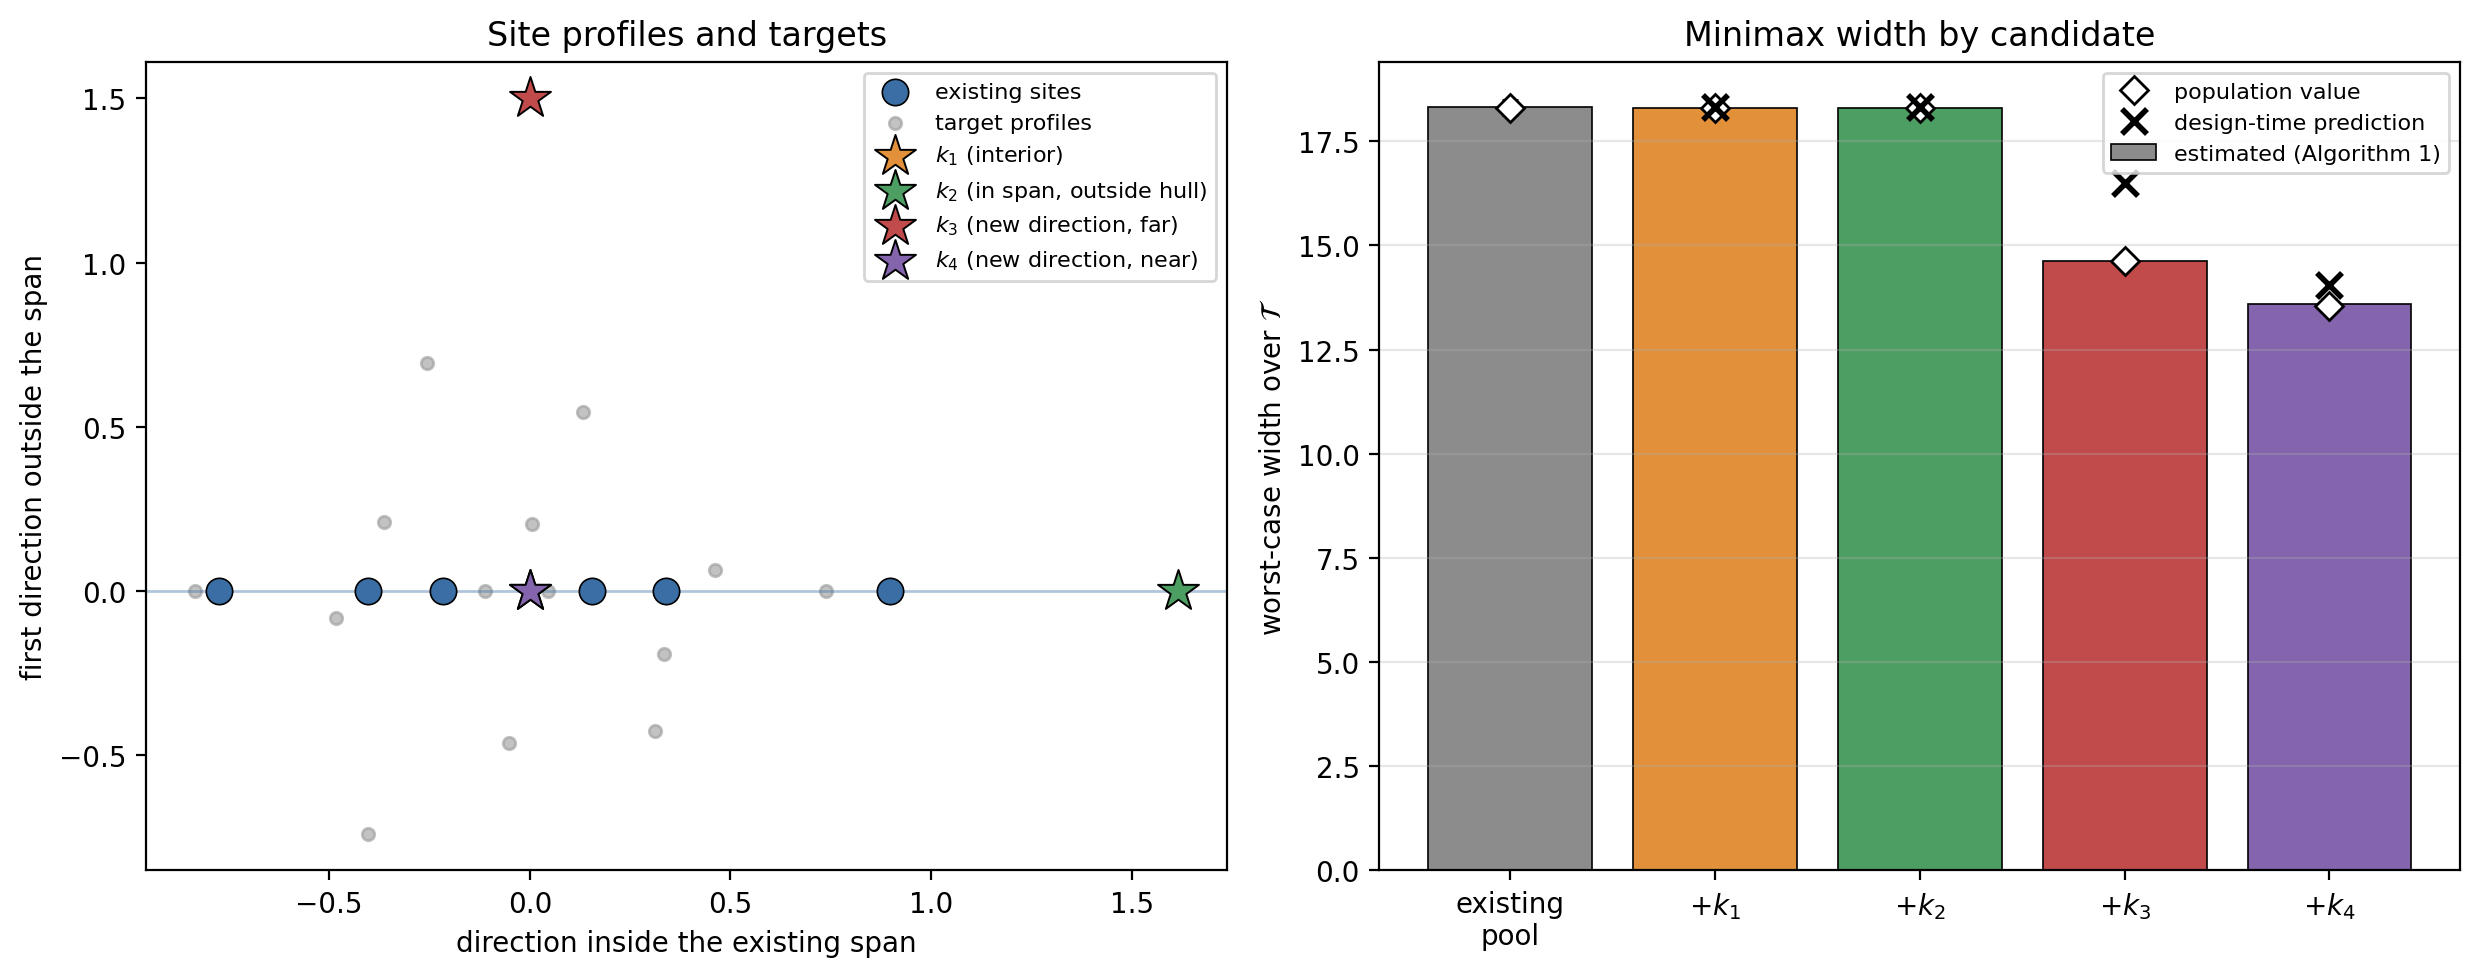
\includegraphics[width=\textwidth]{figure1.png}
  \caption{\textbf{Site selection with estimated bounds.} Left: the
  fixed geometry, projected onto one direction inside the existing span
  and the first direction outside it. Right: worst-case width over the
  target region for the existing pool and after each candidate, showing
  the mean and standard deviation of the estimated widths across 40
  replicates, the exact population width, and the design-time
  prediction computed before the candidate experiment.}
  \label{fig:selection}
\end{figure}

\subsection{The conflict mechanism}
\label{subsec:sim-monotonicity}

The second experiment tests \cref{thm:monotone} and its failure mode.
Two profiles are reused, the in-span candidate $k_2$ and the
hull-expanding candidate $k_3$, and each is added twice: once with
outcomes drawn from the maintained model, labels $a_1$ and $a_3$, and
once with the candidate site's treated-arm mean shifted by a conflict
of size $0.75$ whose sign is drawn at random each replicate, labels
$a_2$ and $a_4$. The restriction box is re-centered at random each
replicate so that it is generically asymmetric around the identified
slice, which is when the translation mechanism of
\cref{sec:monotonicity} can move widths. Population widths and truth
coverage are computed exactly for every drawn box.

\Cref{fig:monotonicity} and its underlying table say three things.
First, the model-consistent additions behave exactly as
\cref{thm:monotone} requires: $a_1$ leaves the population worst-case
width unchanged in all 40 replicates, $a_3$ strictly shrinks it in all
40, with reductions between $1.1$ and $6.7$, and neither ever loses the
truth. Second, the conflicted in-span addition $a_2$ moves the
population worst-case width in both directions, widening it in 45
percent of replicates and narrowing it in 55 percent, by up to $0.71$
either way. The direction is unpredictable in advance, which is the
point of the counterexample. Third, and most important, $a_2$ removes the true target effect from the
population identified set at the span-identified targets in every
replicate, while its worst-case width moves by at most a few percent.
The width does not show the damage, and the interval no longer covers
the true effect. The conflicted hull-expanding addition
$a_4$ still shrinks widths here, and its bias lies in the directions that remain unidentified. This is
why the compatibility screen of \cref{sec:monotonicity}, and not the
width, is the right check for it.

\begin{figure}[t]
  \centering
  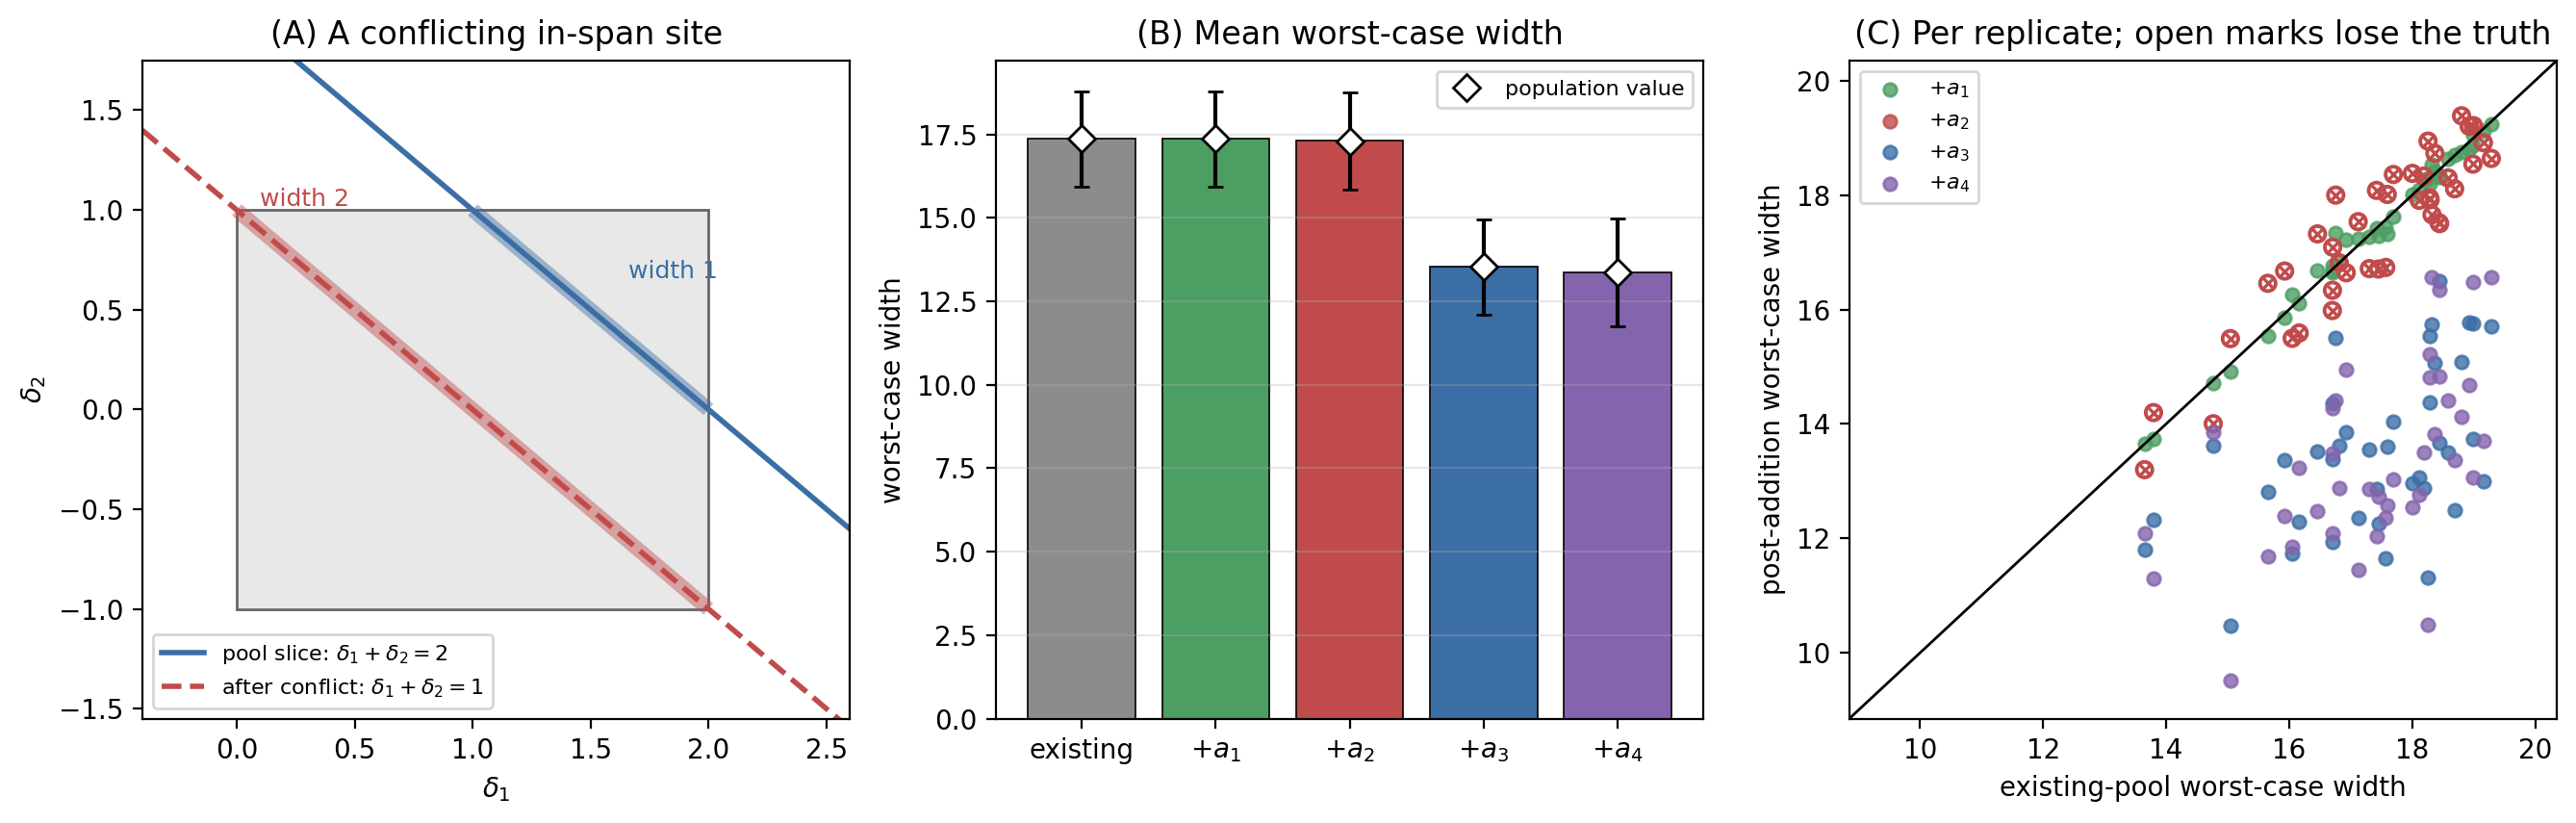
\includegraphics[width=\textwidth]{figure2.png}
  \caption{\textbf{What a conflicting site does.} (A) The two-site
  example of \cref{sec:monotonicity}: a third site on the pool's own
  line whose outcomes conflict with the pool moves the identified slice
  and doubles the width at the target. (B) Mean estimated worst-case
  width across 40 replicates with the exact population value marked.
  (C) Post-addition against existing-pool worst-case width by
  replicate. Open markers are replicates whose population identified
  set no longer covers the true effect at every target: all 40
  replicates of the conflicted in-span addition $a_2$, and none of the
  model-consistent additions.}
  \label{fig:monotonicity}
\end{figure}

\FloatBarrier

\section{Case study: which microcredit experiment was worth running}
\label{sec:case-study}

The microcredit data let us test the design rule against experiments
that have already been run. All seven country experiments were run, so we can
hide one, score it as a candidate from its lending terms alone, and then
reveal its data to check the prediction. This is the forward version of
the leave-one-out exercise in \citet{boyarsky2026}, and it gives a
design rule for future experiments a test it rarely gets, because the
future data already exist.

\subsection{Specification}
\label{subsec:case-spec}

The specification is the one fixed in the companion paper's case study,
and the replication code reproduces every number. The outcome is household revenues. The context basis holds nine
coded terms: promotion, the annual interest rate, and the average loan
size as a share of income, each coded on the source pool's rank scale,
plus their squares and pairwise products, with every column scaled by
its source-pool standard deviation. Unit-level covariates are the six
standardized household variables. Estimation uses the rank consistent
estimator with three folds, boosted outcome and density-ratio fits, and
the regularized multinomial site classifier. The restriction ladder is
the companion paper's: a magnitude cap of $M=888$ revenue units, one
standard deviation of the outcome, on the control surface and on the
treatment shift, then effect ordering at $\kappa=1$, then the sign
restrictions on the interest-rate terms of the treatment shift. We
report the final rung. Coding is frozen at each target's full six-site
source pool, so that removing a source site changes only whose data enter the
moments, and the held-out benchmarks are the covariate-adjusted
design-based estimates with clustering at each country's randomization
unit.

For each target country, Bosnia and Morocco as in the companion paper,
the exercise runs over the six five-site source pools. The missing sixth country is the candidate. Its coded profile is known
and its data are hidden. At design time we run the rank test of \cref{sec:selection},
forecast the revealed scalars with the feasibility-aware neutral
forecast, and solve the width map \eqref{eq:width-map} for the
predicted interval. The neutral forecast sets the new coordinate of the
fixed effects to the value closest to zero that the pool's own
restrictions allow, which applies to two of the Bosnia pools, where the sign restrictions
pin the coordinate away from zero. Then we reveal the
candidate's experiment, refit the estimator on all six source sites, and
compare.

\subsection{Bosnia: a predictable collapse}
\label{subsec:case-bosnia}

Every five-site source pool for Bosnia gives the same result
(\cref{tab:case,fig:case}). The centered profiles of five source sites span
four directions against nine basis terms, the interval at the final
rung is wide and unsigned, with widths between $3{,}525$ and $7{,}291$
revenue units, and no five-site pool supports a conclusion about
Bosnia. The rank test, computed from lending terms alone, reports that
every missing country expands the span. With five source sites and nine
terms, each of the six countries' coded profile lies outside the
five-site hull. The predicted intervals collapse accordingly, with
predicted reductions of 93 to 100 percent, and the realized six-site
interval is $[37.1,\,127.3]$, width $90$, reductions of 97 to 99
percent. An analyst holding any five of these experiments, the lending
terms of the sixth, and no outcome data from it would have been told that the sixth experiment removes almost all of the
width that the restrictions leave, and the realized experiments confirm
this.

The forecast cannot determine the location of the collapsed interval,
and the rows differ in location. For four of the six pools the
neutral forecast is an interior point of what the pool allows, the
predicted intervals have widths of $121$ to $286$, and they sit just
below and above zero. The revealed scalars then place the realized
interval strictly above zero, which is the companion paper's signed
conclusion for Bosnia. For the other two pools, the ones missing India
and Morocco, the pool's sign restrictions pin the forecast coordinate
to a boundary. The predicted intervals degenerate to near points,
$[129.1,\,138.6]$ and $\{67.5\}$, which overstates the collapse but is correct in one respect. Once that
direction is resolved, the restrictions themselves nearly determine the
answer, and they already place it above zero. The realized interval agrees in location and adds
back the width, $90$, that the boundary forecast removed.

\begin{table}[t]
\centering
\small
\begin{tabular}{llrrrrr}
\toprule
target & candidate & base width & predicted & pred.\ gain & realized gain \\
\midrule
Bosnia & Ethiopia    & 4{,}606 & 229 & 95.0\% & 98.0\% \\
Bosnia & India       & 7{,}291 & 10  & 99.9\% & 98.8\% \\
Bosnia & Mexico      & 4{,}109 & 235 & 94.3\% & 97.8\% \\
Bosnia & Mongolia    & 4{,}171 & 286 & 93.2\% & 97.8\% \\
Bosnia & Morocco     & 4{,}398 & 0   & 100.0\% & 97.9\% \\
Bosnia & Philippines & 3{,}525 & 121 & 96.6\% & 97.4\% \\
\midrule
Morocco & Bosnia      & 7{,}770  & 6{,}485 & 16.5\% & 17.4\% \\
Morocco & Ethiopia    & 6{,}767  & 6{,}417 &  5.2\% &  5.2\% \\
Morocco & India       & 8{,}074  & 6{,}482 & 19.7\% & 20.5\% \\
Morocco & Mexico      & 8{,}425  & 6{,}480 & 23.1\% & 23.8\% \\
Morocco & Mongolia    & 10{,}453 & 6{,}487 & 37.9\% & 38.6\% \\
Morocco & Philippines & 8{,}165  & 6{,}487 & 20.5\% & 21.4\% \\
\bottomrule
\end{tabular}
\caption{\textbf{Predicted and realized value of the missing
experiment.} Each row hides one country's experiment from the target's
source pool. Base width is the width of the identified set at the final
restriction rung with five source sites. Predicted is the width after adding
the candidate, computed before its data from the coded lending terms
and the feasibility-aware neutral forecast. Gains are relative to the
base width; the realized gain uses the six-site interval. Widths are
in revenue units.}
\label{tab:case}
\end{table}

\subsection{Morocco: a correct ranking of modest gains}
\label{subsec:case-morocco}

Morocco is the target the companion paper cannot sign, and the design
rule explains why in advance. Even the full six-site source pool leaves
most of Morocco's loading outside the span of the source profiles, so no
single candidate can
deliver a collapse. What the rule can do is rank the six candidates,
and here the check is informative, because each base pool differs and
each realized gain is a different number. The predicted gains run from 5.2
percent for Ethiopia to 37.9 percent for Mongolia. The realized gains
run from 5.2 to 38.6 percent, and they match the predictions candidate
by candidate to within about one percentage point
(\cref{tab:case}). The ranking is exact. Mongolia's experiment, which has the highest
interest rate in the pool and the lending environment most unlike the
others, is the one that helps Morocco most. Ethiopia's experiment, whose
coded terms the other source sites nearly reproduce, adds almost
nothing. An investigator with the five-country pool and the six
candidates' lending terms would have chosen Mongolia, and she would
have been right, for the predicted reason. The rule also reports what none of the candidates fixes. Every predicted
and realized interval for Morocco stays wide and unsigned. Strengthening the Morocco conclusion
requires a site outside the observed hull in Morocco's direction, not a
sixth source site from this pool.

\begin{figure}[t]
  \centering
  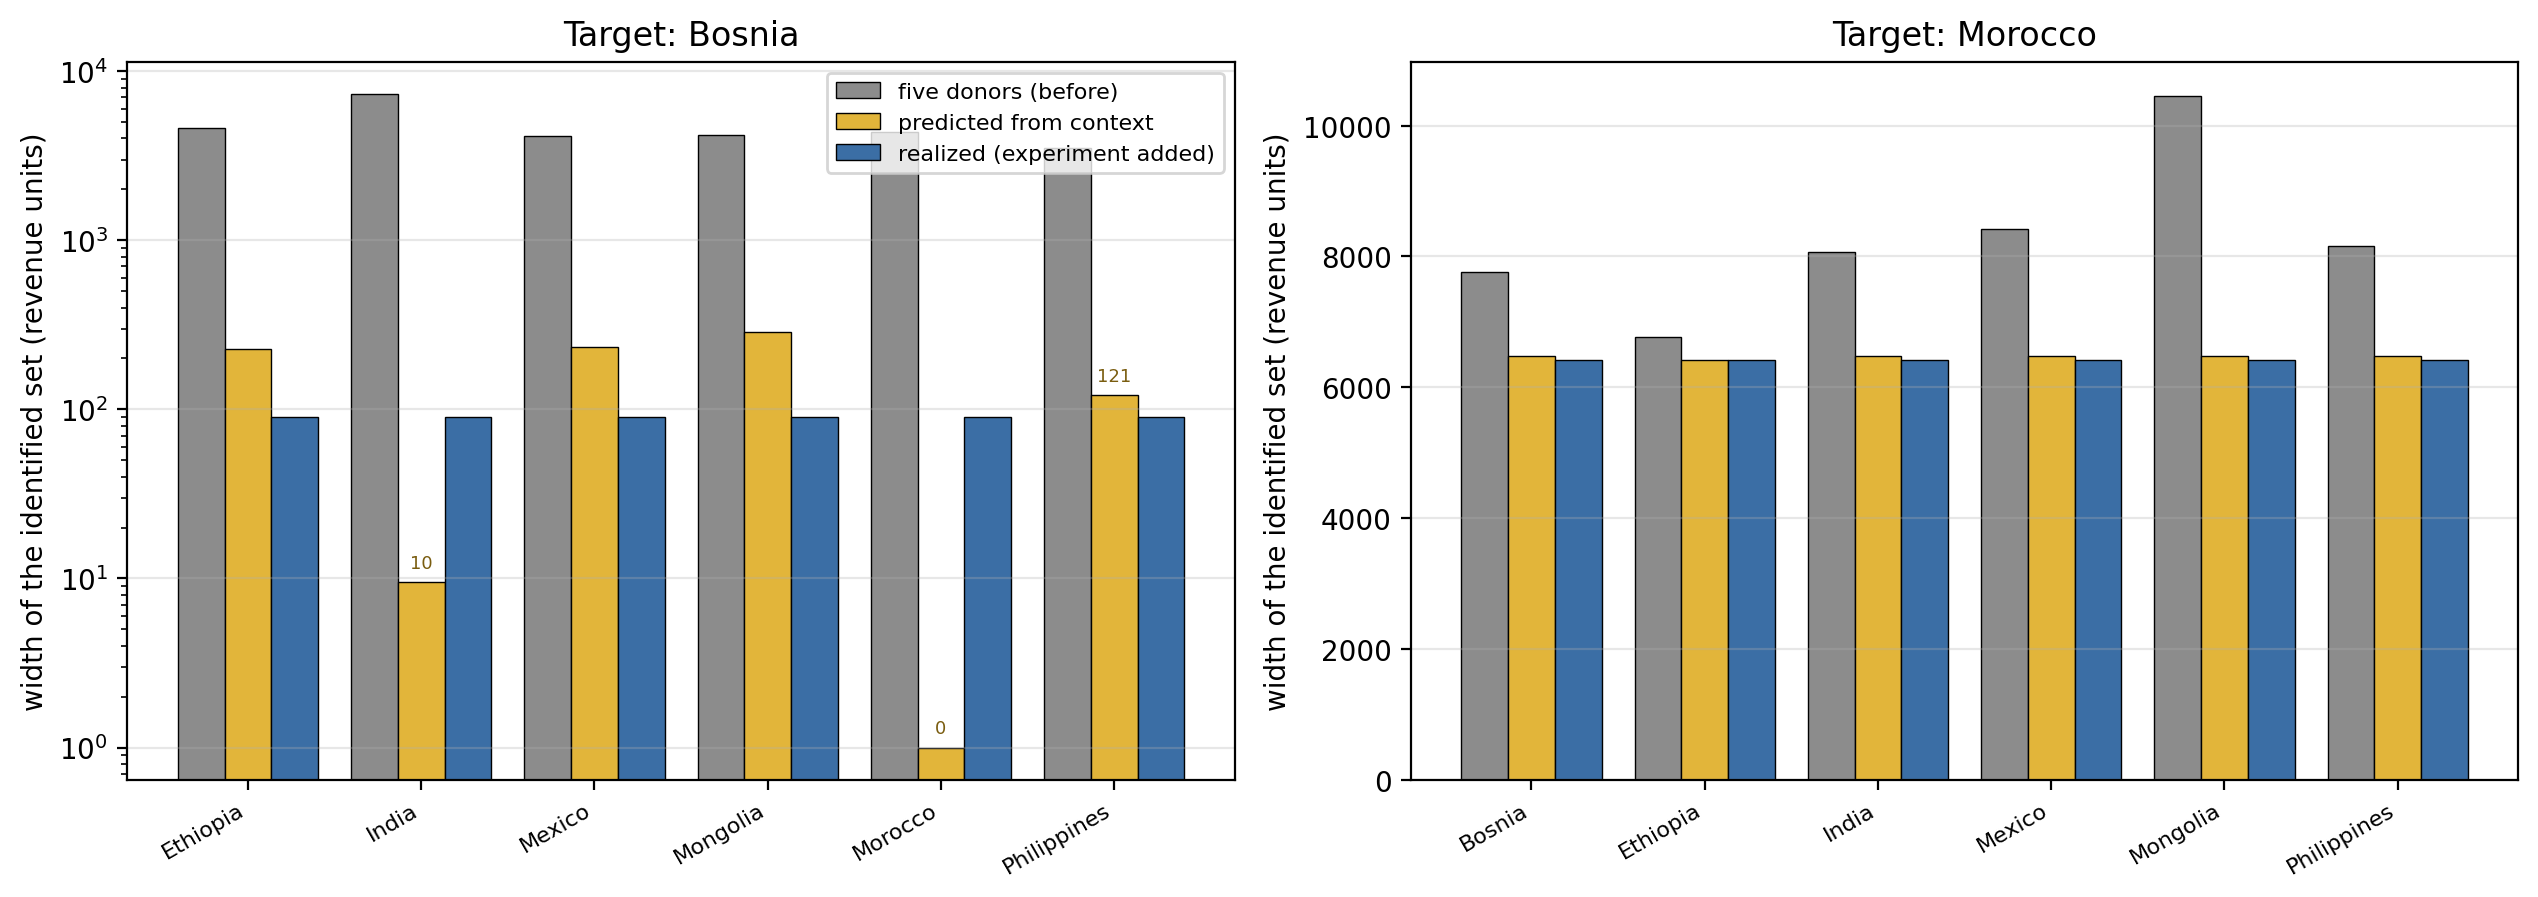
\includegraphics[width=\textwidth]{figure3.png}
  \caption{\textbf{Predict, then check, on the microcredit
  experiments.} For each target and each hidden country: the width of
  the identified set at the final restriction rung with five source sites,
  the width predicted at design time from the hidden country's lending
  terms, and the realized width once its experiment is added. The
  Bosnia panel uses a logarithmic scale because its widths span two
  orders of magnitude, with the near-point predictions labeled.}
  \label{fig:case}
\end{figure}

\subsection{What the exercise does and does not show}
\label{subsec:case-caveats}

Three caveats limit the claim. First, the exercise conditions on the
companion paper's specification: the coded basis, the frozen coding,
and the restriction ladder. The predictions are exact statements about
that specification, not about microcredit at large. Second, the
predictions use estimated base-pool inputs, so they inherit sampling
error; the near-exact match at Morocco partly reflects that base and
augmented fits share five countries of data. Third, the exercise also tests \cref{thm:monotone}. The realized
additions never widened an interval, which is consistent with the
maintained model, and the compatibility screen of \cref{sec:monotonicity} raises no conflict
at the final rung for either target, since the augmented programs
remain feasible. When a screen does fail, as it does on these data for
tighter caps in the supplementary appendix of the companion paper, the
right object to report is the disagreement itself.

\FloatBarrier

\section{Discussion}
\label{sec:discussion}

The sensitivity framework of \citet{boyarsky2026} separates what pooled
experiments identify from what must be assumed. This paper adds the design question. When the answer is a wide interval,
where should the next experiment go? The question is answerable before
the experiment to a larger degree than we expected. Identification
gains are a property of the candidate's context profile relative to the
affine hull of the observed profiles. The bounds after the addition are
computable in advance up to one revealed scalar per treatment arm, with
the forecast error priced by the dual of the added constraint. Under the
maintained model a new site can only refine the set, and when a new site
instead moves conclusions the pool had pinned down, that movement is
evidence against the pooled model, concentrated exactly where the pool
claimed precision. The microcredit exercise suggests that these statements also hold in
finite samples. Computed from lending terms with the companion paper's
estimator, the predictions matched the realized experiments.

Several extensions follow the same lines. Costs enter separably, so a
budgeted rule ranks candidates by predicted gain per unit cost within
the screened pool. Choosing several sites at once is a coverage problem. The identification
gain of a set of candidates is the rank added by their profiles, which
is a matroid rank function, so greedy selection has the usual submodular
guarantee for the identification part. The width objective itself should
be re-solved at the chosen set.
When the candidate's covariate distribution is unknown, the overlap condition of \cref{subsec:augmentation} is the input most
likely to fail, and a
worst-case treatment of the candidate's covariate law would make the
precision part of the score conservative without changing the span
part. Inference for the selected design, as opposed to inference for
the bounds at a fixed design, remains open. The selection is a minimum of a maximum of estimated
program values, and the tools in the
companion paper cover each fixed program but not the selection event.

Two practical lessons follow. First, the design question depends on the choice of context basis. Every statement in this paper is
relative to the chosen context basis, and a candidate that expands the
hull in one coding can be interior in another. The companion paper's
sweeps show how much coding moves identification geometry, and a
selection exercise should be run over the same codings the final
analysis will report. Second, the most useful output of the rule can be a negative result. At Morocco the rule reports that no available candidate
delivers a signed conclusion, and that the useful experiment is one
nobody has run, in a lending environment beyond the observed hull in
Morocco's direction. A design rule that can report that no available candidate helps, and
which direction would help, gives a concrete request for the next trial.


\bibliographystyle{plainnat}
\bibliography{external_validity}

\appendix
\section{Proofs}
\label{app:proofs}

Throughout the appendix, \cref{ass:model} holds for every site that
appears, including candidate sites unless the text says otherwise, and
the eigenvalue condition of \cref{sec:setting} holds for the pool and,
where an augmented pool appears, for the augmented pool. We write
$\Pi_V$ and $\Pi^\perp$ for the orthogonal projections onto $\Vspan$ and
$\Vspan^\perp$, and $\beta^\circ=(\beta_0^\circ,\beta_1^\circ)$ for the
true coefficient vector of \eqref{eq:response-model}. Recall from
\eqref{eq:span} that $\Vspan$ is the span of the centered site profiles
and that $\affhull(\pool)=c_1+\Vspan$.

Two facts from \citet{boyarsky2026} are used repeatedly. First, the
normal equations: under \cref{ass:model}, for any pooled source law
whose sites obey \eqref{eq:response-model} with the same coefficients,
\begin{equation}
  \cov(C,\pseudo{a}\mid X)=\cov(C\mid X)\,\beta_a^\circ
  \quad\text{almost surely, so}\quad
  \dmom{a}=\CovC\beta_a^\circ.
  \label{eq:app-normal}
\end{equation}
Second, under the eigenvalue condition, $\range(\CovC)=\Vspan$ and
$\kernel(\CovC)=\Vspan^\perp$, so the solution set of the equality
system in \eqref{eq:feasible-set} is
$\{\beta_a:\ \CovC\beta_a=\dmom{a}\}
=\beta^\circ_a+\Vspan^\perp$.

\subsection{Proof of \texorpdfstring{\cref{lem:loading}}{Lemma 1}}
\label{app:proof-loading}

\begin{proof}
Write $p_s(x)=\pr_\sP(C=c_s\mid X=x)$, so
$\muC(x)=\sum_{s=1}^S p_s(x)\,c_s$ with $p_s(x)\geq0$ and
$\sum_s p_s(x)=1$ for $\sP$-almost every $x$, hence for $\tP$-almost
every $x$ by overlap. Then
$q:=\E_{\tP}[\muC(X)]=\sum_s \bar w_s c_s$ with $\bar w_s=\E_{\tP}[p_s(X)]\geq0$
and $\sum_s\bar w_s=1$, so $q\in\convhull\{c_1,\ldots,c_S\}\subseteq
\affhull(\pool)$. Since $\affhull(\pool)=c_1+\Vspan$, we have
$q-c_1\in\Vspan$ and therefore
\[
  \Pi^\perp\ellvec=\Pi^\perp(\ct-q)
  =\Pi^\perp(\ct-c_1)-\Pi^\perp(q-c_1)=\Pi^\perp(\ct-c_1).
\]
The distance from a point to the affine set $c_1+\Vspan$ is the norm of
the component of the offset orthogonal to $\Vspan$, which gives
\eqref{eq:loading-distance}. Finally, under the eigenvalue condition
$\range(\CovC)=\Vspan$, so $\ellvec\in\range(\CovC)$ if and only if
$\Pi^\perp\ellvec=0$, if and only if $\Pi^\perp(\ct-c_1)=0$, if and only
if $\ct\in c_1+\Vspan=\affhull(\pool)$.
\end{proof}

\subsection{Proof of \texorpdfstring{\cref{prop:dichotomy}}{Proposition 1}}
\label{app:proof-dichotomy}

\begin{proof}
With $\restrset=\R^{2p}$ the feasible set is the product of the two
equality solution sets, $\feasset=\prod_{a\in\{0,1\}}
(\beta^\circ_a+\Vspan^\perp)$, which contains $\beta^\circ$. For
$\beta_a=\beta^\circ_a+z_a$ with $z_a\in\Vspan^\perp$,
\[
  \ellvec^\top(\beta_1-\beta_0)
  =\ellvec^\top(\beta^\circ_1-\beta^\circ_0)
  +(\Pi^\perp\ellvec)^\top(z_1-z_0),
\]
because $z_1-z_0\in\Vspan^\perp$. If $\ct\in\affhull(\pool)$, then
$\Pi^\perp\ellvec=0$ by \cref{lem:loading}, the objective is constant on
$\feasset$, and both endpoints equal $\psi_T$, so the width is zero. If
$\ct\notin\affhull(\pool)$, then $\Pi^\perp\ellvec\neq0$. Taking
$z_1=t\,\Pi^\perp\ellvec$ and $z_0=0$ with $t\to\pm\infty$ drives the
objective to $\pm\infty$, so the width is infinite.
\end{proof}

\subsection{Proof of \texorpdfstring{\cref{prop:hull}}{Proposition 2}}
\label{app:proof-hull}

\begin{proof}
Write $u=\Pi^\perp(\cand{k}-c_1)$, so
$\cand{k}-c_1=\Pi_V(\cand{k}-c_1)+u$ and
\[
  \Vspan'=\Vspan+\operatorname{span}\{\cand{k}-c_1\}
  =\Vspan+\operatorname{span}\{u\}.
\]
If $u=0$ the two spans coincide. If $u\neq0$ the sum is orthogonal and
$\dim\Vspan'=r+1$; moreover $u=0$ exactly when
$\cand{k}\in c_1+\Vspan=\affhull(\pool)$, which proves the equivalences.
For the complement, $x\in\Vspan'^{\perp}$ if and only if $x\perp\Vspan$
and $x\perp u$, that is $\Vspan'^\perp=\Vspan^\perp\cap\{u\}^\perp$.
Finally, every residual $C-\muC'(X)$ of the augmented pool lies in
$\Vspan'$, because $\muC'(x)$ is a convex combination of the augmented
profiles, so $\range(\CovC')\subseteq\Vspan'$ always, and the augmented
eigenvalue condition states that
$\Bspan'^\top\CovC'\Bspan'$ is positive definite, which forces
$\range(\CovC')=\Vspan'$ and, by symmetry of $\CovC'$,
$\kernel(\CovC')=\Vspan'^{\perp}$.
\end{proof}

\subsection{Proof of \texorpdfstring{\cref{prop:distance}}{Proposition 3}}
\label{app:proof-distance}

\begin{proof}
Only the shift $\shift=\beta_1-\beta_0$ enters the objective and the
restriction, and the pair of equality systems constrains it through
$\CovC\shift=\dmom{1}-\dmom{0}$: given any such $\shift$, choosing
$\beta_0$ with $\CovC\beta_0=\dmom{0}$ and $\beta_1=\beta_0+\shift$
satisfies both systems. The solution set for the shift is
$\bar\shift+\Vspan^\perp$, where $\bar\shift$ is the minimum-norm
solution and lies in $\Vspan$. For $\shift=\bar\shift+\nu$ with
$\nu\in\Vspan^\perp$, orthogonality gives
$\norm{\shift}_2^2=\norm{\bar\shift}_2^2+\norm{\nu}_2^2$, so the cap
$\norm{\shift}_2\leq\tau$ is exactly
$\norm{\nu}_2\leq\rho_\tau:=(\tau^2-\norm{\bar\shift}_2^2)^{1/2}$, and
the objective is
$\ellvec^\top\shift=\ellvec^\top\bar\shift+(\Pi^\perp\ellvec)^\top\nu$.
By the Cauchy--Schwarz inequality, the supremum and infimum of
$(\Pi^\perp\ellvec)^\top\nu$ over the ball of radius $\rho_\tau$ in
$\Vspan^\perp$ are $\pm\rho_\tau\norm{\Pi^\perp\ellvec}_2$, attained at
$\nu=\pm\rho_\tau\,\Pi^\perp\ellvec/\norm{\Pi^\perp\ellvec}_2$ when
$\Pi^\perp\ellvec\neq0$ and trivially when it is zero. The width is
therefore $2\rho_\tau\norm{\Pi^\perp\ellvec}_2$, and
\cref{lem:loading} identifies the last factor with
$\dist(\ct,\affhull(\pool))$.
\end{proof}

\subsection{Proof of \texorpdfstring{\cref{prop:refinement}}{Proposition 4}}
\label{app:proof-refinement}

\begin{proof}
Apply \eqref{eq:app-normal} to the augmented pool: because the candidate
site obeys \eqref{eq:response-model} with the same coefficients,
$\dmom{a}'=\CovC'\beta^\circ_a$, so the augmented equality solution set
is $\beta^\circ_a+\kernel(\CovC')$, and by \cref{prop:hull} this kernel
is $\Vspan^\perp\cap\{\newdir{k}\}^\perp$ in the hull-expanding case and
$\Vspan^\perp$ in the rank-preserving case.

In the rank-preserving case the solution sets coincide with the pool's,
so $\feasset'=\feasset$ after intersecting with $\restrset$. In the
hull-expanding case, for $\beta_a=\beta^\circ_a+z_a$ with
$z_a\in\Vspan^\perp$ we have
$\newdir{k}^\top\beta_a=\newdir{k}^\top\beta^\circ_a
+\newdir{k}^\top z_a$, and $z_a\in\{\newdir{k}\}^\perp$ exactly when
$\newdir{k}^\top\beta_a=\newdir{k}^\top\beta^\circ_a=\reveal{a}{k}$.
Hence
\[
  \beta^\circ_a+\kernel(\CovC')
  =\bigl(\beta^\circ_a+\Vspan^\perp\bigr)
  \cap\bigl\{\beta_a:\ \newdir{k}^\top\beta_a=\reveal{a}{k}\bigr\},
\]
and intersecting both arms' sets with $\restrset$ gives
\eqref{eq:refinement}. The scalar $\reveal{a}{k}$ is a linear functional
of $\Bspan'^\top\beta^\circ_a$, which the augmented pool identifies
through its normal equations because $\newdir{k}\in\Vspan'$; it is not
identified by the pool alone because moving $\beta_a$ along
$\newdir{k}\in\Vspan^\perp$ leaves every pool moment unchanged.

For the last claim, compare the augmented-pool endpoint programs, which
use $(\bT',\ellvec')$, with the base-objective programs over
$\feasset'$. Write $q=\E_{\tP}[\muC(X)]$ and $q'=\E_{\tP}[\muC'(X)]$ for
the two mixture points. As in the proof of \cref{lem:loading}, $q$ lies
in $\affhull(\pool)$ and $q'$ in $\affhull(\pool\cup\{k\})$, so
$\ellvec-\ellvec'=q'-q\in\Vspan'$, and for every $\beta\in\feasset'$,
writing $\shift=\beta_1-\beta_0=\shift^\circ+\nu$ with
$\nu\in\Vspan'^\perp$,
\[
  (\ellvec-\ellvec')^\top\shift
  =(\ellvec-\ellvec')^\top\shift^\circ
\]
is constant on $\feasset'$. Both decompositions represent the same
target effect, $\psi_T=\bT+\ellvec^\top\shift^\circ
=\bT'+\ellvec'^\top\shift^\circ$, so
$\bT'-\bT=(\ellvec-\ellvec')^\top\shift^\circ$, and for every
$\beta\in\feasset'$,
\[
  \bT'+\ellvec'^\top\shift
  =\bT+(\ellvec-\ellvec')^\top\shift^\circ
  +\ellvec^\top\shift-(\ellvec-\ellvec')^\top\shift
  =\bT+\ellvec^\top\shift .
\]
The two programs have the same objective value at every feasible point,
hence the same endpoints.
\end{proof}

\subsection{Proof of \texorpdfstring{\cref{prop:omitted-bias}}{Proposition on omitted-moderator bias}}
\label{app:proof-omitted-bias}

\begin{proof}
Write $\widetilde C=C-\muC(X)$ and
$\widetilde U=U-\muU(X)$. Randomization and
\eqref{eq:omitted-response-model} imply
\[
  \cov\bigl(C,\pseudo{1}-\pseudo{0}\mid X\bigr)
  =\cov(C\mid X)\theta+\cov(C,U\mid X)\gamma.
\]
Taking expectations gives \eqref{eq:omitted-moment-shift}. Let
$q=\CUcov\gamma$. Every solution of \eqref{eq:omitted-normal-equation} has
the form
\[
  \theta^C=\theta+\CovC^\dagger q+z,
  \qquad z\in\kernel(\CovC),
\]
because $q\in\Vspan=\range(\CovC)$. The true target effect is
\[
  \psi_T=\bT+\ellvec^\top\theta+\ellU^\top\gamma,
\]
which follows by averaging \eqref{eq:omitted-response-model} over the target
covariate law. If $\ct\in\affhull(\pool)$, then
$\ellvec\in\range(\CovC)$ by \cref{lem:loading}, so
$\ellvec^\top z=0$. Subtracting
$\psi_T^C=\bT+\ellvec^\top\theta^C$ gives
\eqref{eq:omitted-bias}.
\end{proof}

\subsection{Proof of \texorpdfstring{\cref{thm:omitted-refinement}}{Theorem on omitted-moderator refinement}}
\label{app:proof-omitted-refinement}

\begin{proof}
Subtract the affine combination of the source conditional treatment
responses from the candidate response. The $g_\Delta(x)$ terms cancel because
$\sum_s w_s=1$, and the context terms cancel because
$\cand{k}=\sum_s w_sc_s$. The remaining term is
\[
  \left(u_k-\sum_s w_su_s\right)^\top\gamma
  =\udisc{k}^\top\gamma,
\]
which proves \eqref{eq:omitted-contrast}.

The candidate's observed contrast therefore adds exactly the equality
$\udisc{k}^\top\gamma=\rho_k$ to the source moment and restriction system,
which proves \eqref{eq:omitted-feasible-update}. The true parameter belongs to
both sets by assumption, so the candidate set is a subset of the source set
and both contain the truth. The infimum of the target functional can only
increase and its supremum can only decrease after intersecting with this
hyperplane, proving \eqref{eq:omitted-monotonicity}. If $\udisc{k}=0$, the
contrast is zero under the model and the added equality is redundant, so the
sets and widths are equal. If the hyperplane cuts a target-relevant direction,
one of the endpoint programs changes strictly.
\end{proof}

\subsection{Proof of \texorpdfstring{\cref{thm:monotone}}{Theorem 1}}
\label{app:proof-monotone}

\begin{proof}
By \cref{prop:refinement}, $\feasset'$ is either $\feasset$ or
$\feasset$ intersected with the two hyperplanes through
$\beta^\circ$, so $\feasset'\subseteq\feasset$ in both cases. The true
vector $\beta^\circ$ satisfies the equality systems of both pools by
\eqref{eq:app-normal} and lies in $\restrset$ by hypothesis, so
$\beta^\circ\in\feasset'$ and both programs are feasible. By
\cref{prop:refinement} the augmented-pool endpoints equal the base
objective optimized over $\feasset'$, so shrinking the feasible set
weakly raises the infimum and weakly lowers the supremum at every
target, which is \eqref{eq:monotone}, with equality throughout in the
rank-preserving case where $\feasset'=\feasset$. Since
$\beta^\circ\in\feasset'$, the value
$\psi_T=\bT+\ellvec^\top(\beta^\circ_1-\beta^\circ_0)$ lies between the
augmented endpoints.
\end{proof}

\subsection{The dual price of the forecast}
\label{app:dual-price}

For completeness we record the sensitivity statement behind
\eqref{eq:dual-pricing}. Fix one polyhedral branch and a target, and
consider the lower endpoint program of \eqref{eq:width-map} as a
function of the added right-hand side $y=(y_0,y_1)$,
\[
  v_-(y)=\bT+\min_{\beta}\bigl\{\ellvec^\top(\beta_1-\beta_0):\
  \CovC\beta_a=\dmom{a},\
  \newdir{k}^\top\beta_a=y_a,\ a\in\{0,1\},\ G\beta\leq h\bigr\}.
\]
This is a linear program whose right-hand side is affine in $y$, so
$v_-$ is a piecewise linear convex function of $y$ on its feasibility
domain, and standard linear-programming duality gives, at any $y$ where
the optimal basis is unique, $\partial v_-/\partial y_a
=\lambda^{u}_{-,a}$, the optimal multiplier on the row
$\newdir{k}^\top\beta_a=y_a$ \citep[Chapter~4]{bonnans2013perturbation}.
The upper endpoint is the corresponding concave value with multipliers
$\lambda^{u}_{+,a}$. At a kink, the left and right slopes are the
extreme multipliers, and the exact range of predicted intervals over
$|y_a-\what y_a|\leq B$ is obtained by re-solving the two programs at
the corners, which is how the simulations and the case study evaluate
forecast uncertainty. For a finite union of branches the value is the
minimum or maximum of finitely many such functions and the same
statements hold branchwise.




\end{document}
